\begin{frame}
\frametitle{Separation of Concerns}
\begin{block}{Different expertise, different focus}
Relevant pieces of code should be easy to divide
\end{block}
\begin{itemize}
\item Much like any library -- clients control behavior by passing
  arguments, not modifying implementation
\item Can be very flexible -- arguments with behavior of their own
  (e.g., functors)
\item Several examples: initial mapping schemes, dynamic load
  balancing strategies
\item CS-specialist logic doesn't pollute application code, can be
  swapped out with minimal effort
\item Location-independent algorithm expression and runtime-mediated
  execution are essential enabling features
\end{itemize}
\end{frame}


\begin{frame}
\frametitle{Different expertise, different focus}
\framesubtitle{Mapping Example: Quantum Chemistry with {\sc OpenAtom}}
Replace with illustration of OpenAtom arrays
\end{frame}

\begin{frame}
\frametitle{Different expertise, different focus}
\framesubtitle{Mapping Example: Quantum Chemistry with {\sc OpenAtom}}
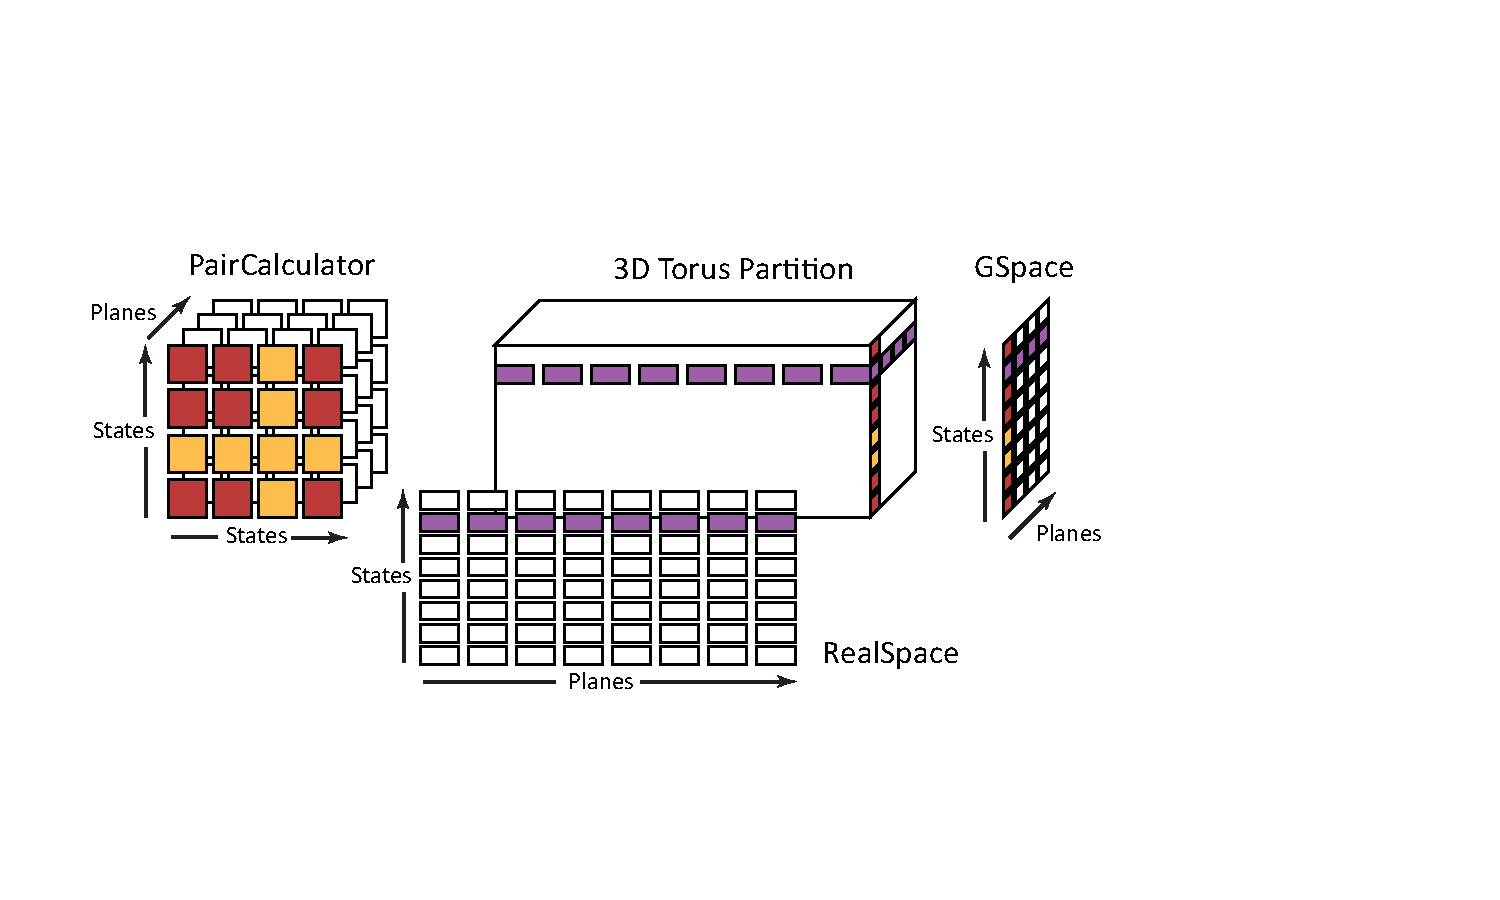
\includegraphics[width=0.9\textheight]{../figures/openatom/mapping.pdf}
\end{frame}


\begin{frame}
\frametitle{Different expertise, different focus}
\framesubtitle{Mapping Example: Quantum Chemistry with {\sc OpenAtom}}
\includegraphics[width=0.9\textwidth]{../figures/openatom/map.pdf}
\begin{block}{40\% improvement, application only changed in initialization!}\end{block}
\end{frame}


\begin{frame}
\frametitle{Separation of Concerns}
\begin{block}{Layered responsibility}
Application worries about \emph{what}, runtime system worries about \emph{how}
\end{block}
\begin{itemize}
\item What data to send, vs. message allocation and packing
\item Who to talk to, vs. where they live
\end{itemize}
\end{frame}
